\documentclass{standalone}
\usepackage{tikz}
\usetikzlibrary{decorations.pathmorphing,patterns}
\begin{document}
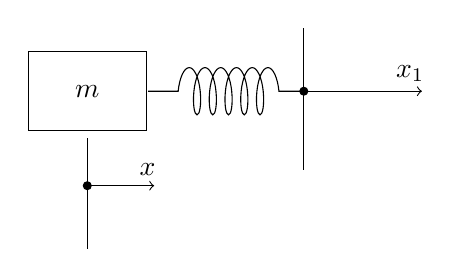
\begin{tikzpicture}
\draw  (0,0) rectangle (1.5,1)  node[pos=0.5] {$m$};
\draw (0.75,-0.1) -- (0.75,-1.5);
\draw [fill] (0.75,-0.7) circle (0.05);
\draw [->] (0.75,-0.7) -- (1.6,-0.7) node[above, pos=0.9] {$x$};
\node (a) at (1.4,0.5) {};
%\node[circle,fill=blue,inner sep=2.5mm] (a) at (0,0) {};
%\node[circle,fill=blue,inner sep=2.5mm] (b) at (2,2) {};
\draw[decoration={aspect=0.3, pre length = 3.8mm, post length =3mm, segment length=2mm, amplitude=3mm,coil},decorate] (a) -- (3.5,0.5); 
%\draw[decoration={aspect=0.3, segment length=1.5mm, amplitude=3mm,coil},decorate] (2,5) -- (b); 
%\fill [pattern = north east lines] (-1,5) rectangle (3,5.2);
%\draw[thick] (-1,5) -- (3,5);
\draw (3.5,1.3) -- (3.5,-0.5);
\draw [fill] (3.5,0.5) circle (0.05);
\draw [->] (3.5,0.5) -- (5,0.5) node[above, pos=0.9] {$x_{1}$};
\end{tikzpicture}
\end{document}